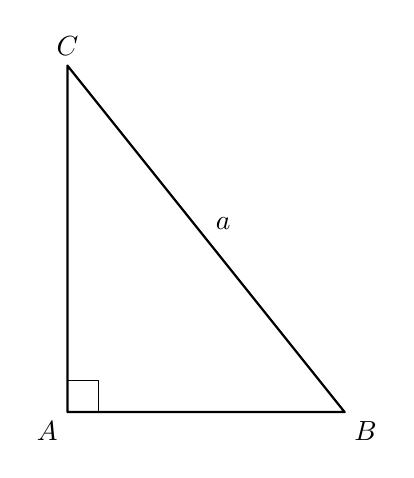
\begin{tikzpicture}[scale=2.2, line join=round, line cap=round]
  \coordinate (A) at (0, 0);
  \coordinate (B) at (1.6, 0);
  \coordinate (C) at (0, 2.0);

  % 绘制直角三角形
  \draw[thick] (A) -- (B) -- (C) -- cycle;

  % 直角标记
  \draw[thin] (0, 0.18) -- (0.18, 0.18) -- (0.18, 0);

  % 顶点与边长标注
  \node[below left] at (A) {$A$};
  \node[below right] at (B) {$B$};
  \node[above] at (C) {$C$};
  \node[above right] at (0.8, 1.0) {$a$};
\end{tikzpicture}
